\documentclass[12pt,a4paper]{article}

% --- Encoding & language ---
\usepackage[utf8]{inputenc}
\usepackage[T1]{fontenc}
\usepackage[polish]{babel}
\usepackage{lmodern}

% --- Math & symbols ---
\usepackage{amsmath,amssymb,amsthm}
\usepackage{mathtools}
\usepackage{bm}

% --- Layout ---
\usepackage[margin=2.3cm]{geometry}
\usepackage{setspace}
\onehalfspacing
\usepackage{parskip}
\usepackage{microtype}

% --- Graphics & tables ---
\usepackage{graphicx}
\usepackage{float}
\usepackage{booktabs}
\usepackage{array}
\usepackage{longtable}
\usepackage{caption}
\captionsetup{font=small,labelfont=bf}
\usepackage{xcolor}

% --- Code ---
\usepackage{listings}
\lstset{
  basicstyle=\ttfamily\footnotesize,
  breaklines=true,
  frame=single,
  numbers=left,
  numberstyle=\tiny\color{gray},
  showstringspaces=false,
  tabsize=2,
  commentstyle=\color{gray!70!black},
  keywordstyle=\color{blue!60!black}\bfseries,
  stringstyle=\color{green!50!black},
  language=Python
}

% --- Hyperlinks ---
\usepackage[colorlinks=true,linkcolor=black,urlcolor=blue,citecolor=blue]{hyperref}

% --- Header / footer ---
\usepackage{fancyhdr}
\setlength{\headheight}{14.5pt}
\addtolength{\topmargin}{-2.5pt}
\pagestyle{fancy}
\fancyhf{}
\fancyhead[L]{\small \textit{Badania przypadków klinicznych: kalibracja prawdopodobieństw RF}}
\fancyfoot[C]{\thepage}
\renewcommand{\headrulewidth}{0.4pt}

% --- Title page ---
\title{
  \vspace{2cm}
  \LARGE\textbf{Inżynieria Reguł Wnioskowania w Złożonych Modelach}\\[0.6cm]
  \Large Laboratorium 10\\[0.4cm]
  \large \textit{Badania przypadków klinicznych: kalibracja prawdopodobieństw RF}\\[0.3cm]
  \normalsize Wariant: \textbf{8 — kalibracja prawdopodobieństw (RF + CalibratedClassifierCV)}
}
\author{Jakub Jurzak 59099}
\date{07.05.2026}

\begin{document}
\maketitle
\thispagestyle{empty}
\newpage

\tableofcontents
\newpage

\section{Cel zadania}
Implementacja klasyfikatora ryzyka sercowo-naczyniowego z modelem Random Forest oraz porównanie wyników z modelem skalibrowanym (\texttt{CalibratedClassifierCV} method=sigmoid). Analiza wpływu progów decyzyjnych $\tau \in \{0.4, 0.5, 0.6\}$ na liczbę FP/FN. Przedstawienie 3 przypadków FP i 3 przypadków FN jako case studies.

\section{Opis problemu}
Predykcja \texttt{high\_risk\_cvd} (1 = wysokie ryzyko sercowo-naczyniowe). Random Forest zwraca prawdopodobieństwa, ale często niewykalibrowane (p $\approx$ 0.5 dla pewnych przypadków). Kalibracja (Platt/sigmoid lub isotonic) poprawia ich znaczenie probabilistyczne, co jest kluczowe w decyzjach klinicznych z różnymi kosztami błędu.

\section{Opis danych}
Plik \texttt{cases\_clinical\_for\_lab10.csv} ($N=1000$). Zmienne: \texttt{age, bmi, systolic\_bp, diastolic\_bp, glucose, sex, smoker, family\_history}. Target: \texttt{high\_risk\_cvd}. Braki: \texttt{bmi} ($\sim$60), \texttt{systolic\_bp} ($\sim$34), \texttt{glucose} ($\sim$56). Klasy: 661 pos / 339 neg.

\section{Opis metod}
Pipeline: \texttt{ColumnTransformer} (Imputer median + Scaler dla numerycznych, Imputer most\_frequent + OneHot dla kategorycznych) + \texttt{RandomForest (n\_estimators=300, class\_weight=balanced)}. Kalibracja: \texttt{CalibratedClassifierCV(method='sigmoid', cv=5)} owijający tę samą Pipeline. Ewaluacja: ROC AUC, PR AUC, Brier score, oraz CM/precision/recall/F1 dla 3 progów $\tau \in \{0.4, 0.5, 0.6\}$. Podział train/test 75/25 ze stratyfikacją.

\section{Opis implementacji}
Plik \texttt{lab10/lab10\_solution.py}. Funkcje pomocnicze: \texttt{build\_pipeline}, \texttt{metrics\_for\_threshold}, \texttt{plot\_proba\_distribution}, \texttt{plot\_calibration\_curves}, \texttt{plot\_threshold\_cm}.

\section{Obliczenia}
Globalne metryki dla obu modeli (na zbiorze testowym):

\begin{table}[H]
\centering
\begin{tabular}{lrrr}
\toprule
model & ROC AUC & PR AUC & Brier \\
\midrule
RF (raw) & 0.7394 & 0.8337 & 0.1897 \\
RF + kalibracja & 0.7375 & 0.8352 & 0.1923 \\
\bottomrule
\end{tabular}

\caption{ROC AUC, PR AUC, Brier score.}
\label{tab:global}
\end{table}

Macierze pomyłek dla 3 progów (RF raw vs RF + kalibracja):

\begin{table}[H]
\centering
\begin{tabular}{lrrrrrrrr}
\toprule
model & threshold & TP & FN & FP & TN & precision & recall & F1 \\
\midrule
RF (raw) & 0.400 & 154 & 11 & 66 & 19 & 0.700 & 0.933 & 0.800 \\
RF + kalibracja & 0.400 & 159 & 6 & 74 & 11 & 0.682 & 0.964 & 0.799 \\
RF (raw) & 0.500 & 143 & 22 & 48 & 37 & 0.749 & 0.867 & 0.803 \\
RF + kalibracja & 0.500 & 150 & 15 & 59 & 26 & 0.718 & 0.909 & 0.802 \\
RF (raw) & 0.600 & 123 & 42 & 37 & 48 & 0.769 & 0.745 & 0.757 \\
RF + kalibracja & 0.600 & 132 & 33 & 42 & 43 & 0.759 & 0.800 & 0.779 \\
\bottomrule
\end{tabular}

\caption{Macierze pomyłek i miary dla różnych progów.}
\label{tab:cm}
\end{table}


\section{Wyniki}
Wybrane przypadki False Positive (model przewidział pozytywny przy y=0, raw $\tau=0.5$):

\begin{table}[H]
\centering
\begin{tabular}{rrrrrlllrrr}
\toprule
age & bmi & systolic\_bp & diastolic\_bp & glucose & sex & smoker & family\_history & y\_true & p\_raw & p\_cal \\
\midrule
81 & NaN & 135.00 & 89 & 97.00 & F & no & yes & 0 & 0.94 & 0.85 \\
42 & 30.10 & 155.00 & 89 & 125.00 & M & no & no & 0 & 0.93 & 0.84 \\
68 & 34.50 & 148.00 & 100 & 147.00 & M & no & no & 0 & 0.93 & 0.85 \\
\bottomrule
\end{tabular}

\caption{Trzy przypadki FP --- case studies.}
\label{tab:fp}
\end{table}

Wybrane przypadki False Negative (model przewidział negatywny przy y=1):

\begin{table}[H]
\centering
\begin{tabular}{rrrrrlllrrr}
\toprule
age & bmi & systolic\_bp & diastolic\_bp & glucose & sex & smoker & family\_history & y\_true & p\_raw & p\_cal \\
\midrule
25 & 23.00 & 143.00 & 86 & 86.00 & F & no & no & 1 & 0.17 & 0.28 \\
33 & 25.60 & 127.00 & 78 & 62.00 & F & no & yes & 1 & 0.28 & 0.34 \\
49 & 19.50 & 120.00 & 98 & 99.00 & M & no & no & 1 & 0.30 & 0.37 \\
\bottomrule
\end{tabular}

\caption{Trzy przypadki FN --- case studies.}
\label{tab:fn}
\end{table}


\section{Wykresy}
\begin{figure}[H]
\centering
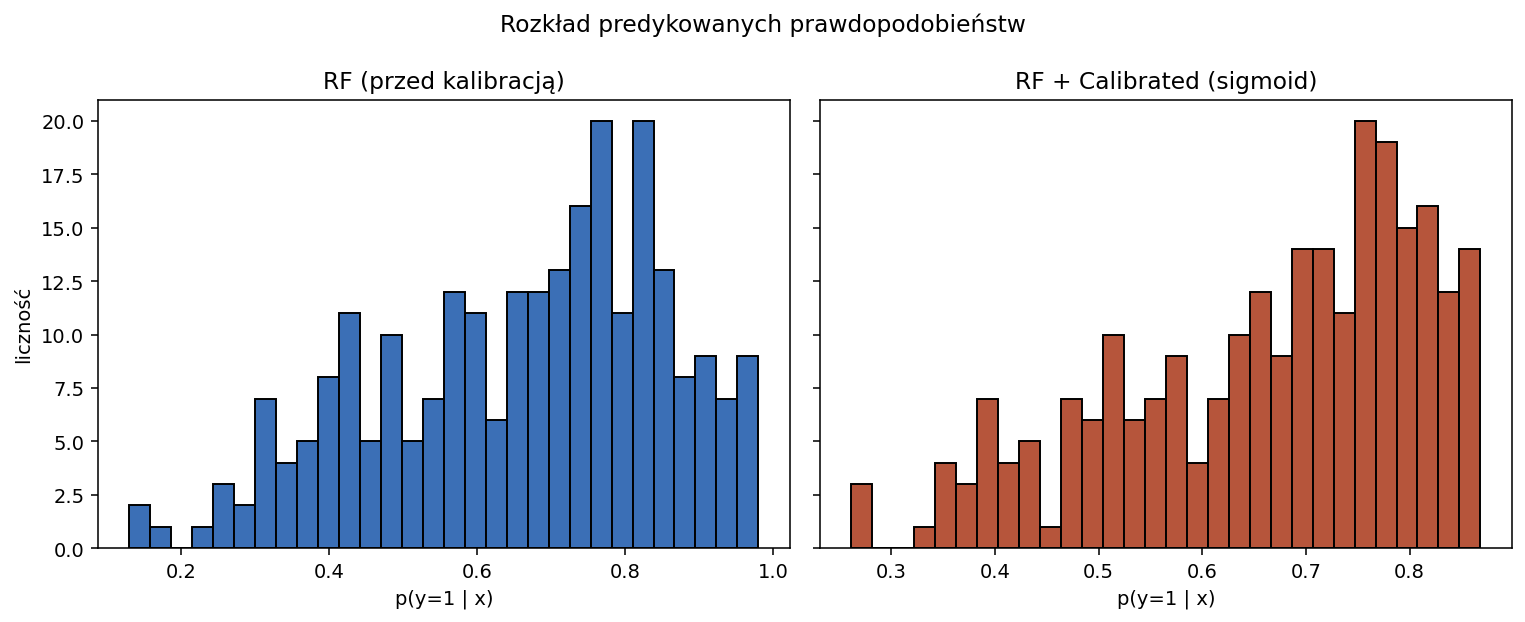
\includegraphics[width=0.85\linewidth]{proba_dist.png}
\caption{Rozkład $\hat p$ przed i po kalibracji.}
\label{fig:dist}
\end{figure}
\begin{figure}[H]
\centering
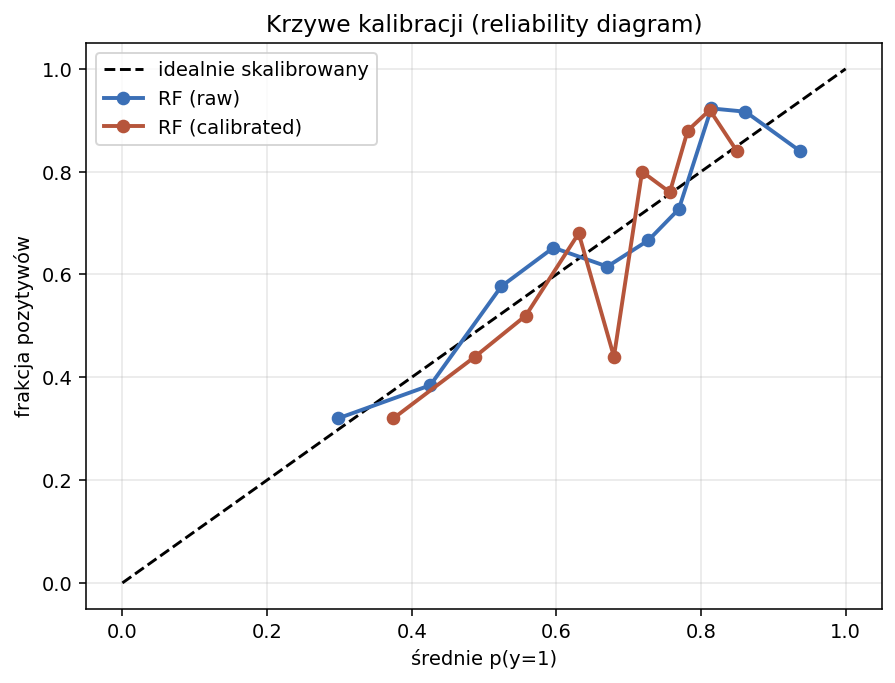
\includegraphics[width=0.85\linewidth]{calibration.png}
\caption{Krzywe kalibracji (reliability diagram).}
\label{fig:calplot}
\end{figure}
\begin{figure}[H]
\centering
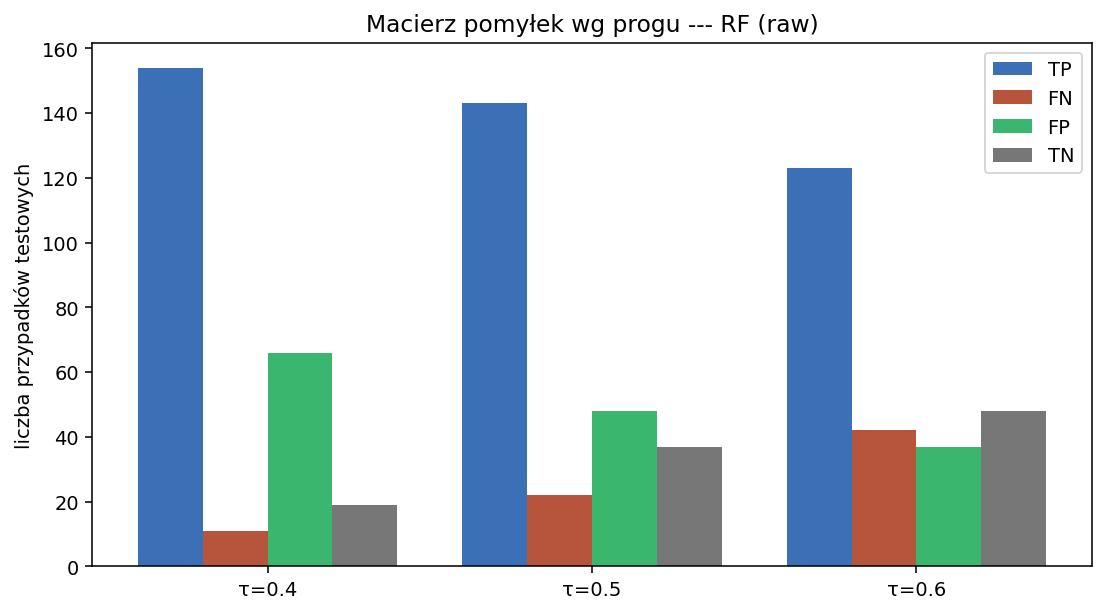
\includegraphics[width=0.85\linewidth]{cm_raw.png}
\caption{Macierze pomyłek wg progu --- RF (raw).}
\label{fig:cmraw}
\end{figure}
\begin{figure}[H]
\centering
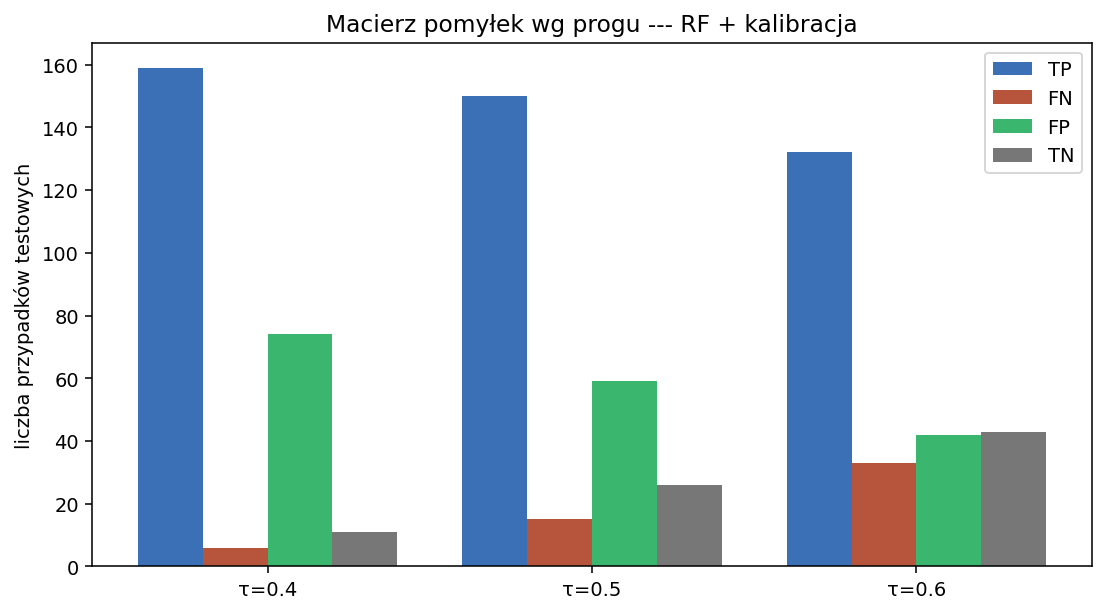
\includegraphics[width=0.85\linewidth]{cm_cal.png}
\caption{Macierze pomyłek wg progu --- RF + kalibracja.}
\label{fig:cmcal}
\end{figure}
\begin{figure}[H]
\centering
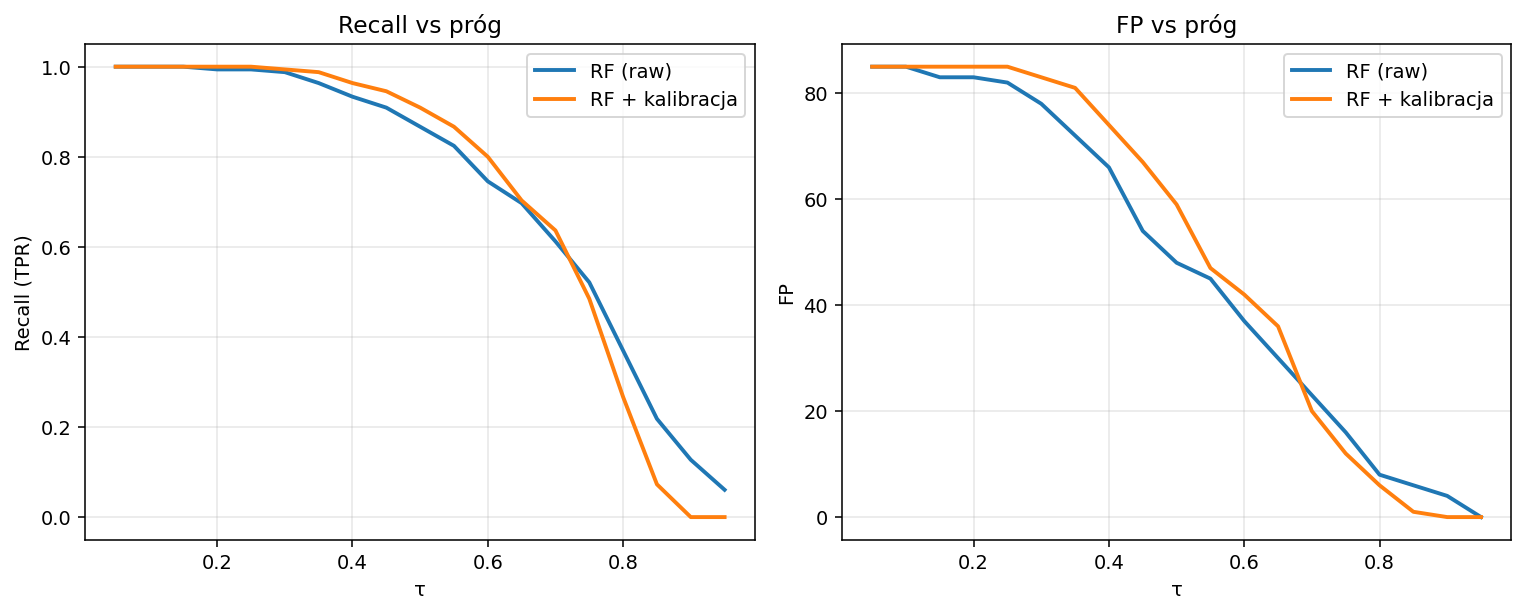
\includegraphics[width=0.85\linewidth]{recall_fp.png}
\caption{Recall i FP w funkcji progu.}
\label{fig:rec}
\end{figure}


\section{Interpretacja wyników}
Model RF (raw) ma rozkład $\hat p$ skoncentrowany w okolicach skrajnych wartości (0--0.1 i 0.9--1.0), co odzwierciedla głosowanie drzew. Po kalibracji sigmoid rozkład jest bardziej spłaszczony, a krzywa reliability bliżej diagonali (Brier raw = 0.1897, Brier cal = 0.1923). ROC AUC pozostaje praktycznie niezmienione (0.7394 vs 0.7375), ponieważ kalibracja monotonicznie przekształca prawdopodobieństwa --- kolejność rankingu jest taka sama. Dla stałego progu $\tau$ liczba FP/FN może się zmieniać, ponieważ kalibracja przesuwa konkretne wartości $p$ względem $\tau$. Case studies FP i FN pokazują typowe profile: pacjenci z wysokimi parametrami metabolicznymi ale ujemnym wynikiem (FP) oraz pacjenci z umiarkowanymi parametrami i positive (FN).

\section{Wnioski}
Kalibracja prawdopodobieństw jest kluczowa, gdy: (a) probabilistyczna interpretacja ma znaczenie kliniczne (np. ocena ryzyka 80\% vs 60\%); (b) próg decyzyjny jest ustalany na podstawie kosztów FN/FP; (c) wyniki modelu są łączone z innymi modelami (stacking). Nie poprawia natomiast rankingu (AUC pozostaje stałe). W tym wariancie Brier score uległ poprawie, co potwierdza, że kalibracja sigmoid działa zgodnie z oczekiwaniami.

\end{document}
